% BHU PYQ -- Professional Exam Template
\documentclass[11pt,a4paper]{article}

\usepackage[a4paper,top=2.5cm,bottom=2.5cm,left=2.8cm,right=2.8cm,headheight=14pt]{geometry}
\usepackage{amsmath,amssymb}
\usepackage[T1]{fontenc}
\usepackage[utf8]{inputenc}
\usepackage{lmodern}
\usepackage{microtype}
\usepackage{fancyhdr}
\usepackage{enumitem}
\usepackage{hyperref}
\usepackage{lastpage}
\usepackage{parskip}
\usepackage{tikz}
\usetikzlibrary{arrows.meta,shapes,positioning}

\hypersetup{colorlinks=true,urlcolor=black,linkcolor=black,
  pdftitle={B.Sc. (Hons.) Zoology Sem-III ZOB-301 -- BHU PYQ}}

\pagestyle{fancy}
\fancyhf{}
\renewcommand{\headrulewidth}{0.4pt}
\renewcommand{\footrulewidth}{0.4pt}
\fancyhead[L]{\small\textit{Banaras Hindu University}}
\fancyhead[R]{\small\textit{Zoology Paper: ZOB-301}}
\fancyfoot[C]{\small Page \thepage\ of \pageref{LastPage}}

\newlist{parts}{enumerate}{3}
\setlist[parts,1]{label=(\Alph*),leftmargin=*,itemsep=4pt,topsep=3pt}
\setlist[parts,2]{label=(\roman*),leftmargin=*,itemsep=2pt,topsep=2pt}
\setlist[parts,3]{label=(\alph*),leftmargin=*,itemsep=2pt,topsep=2pt}
\newcommand{\pts}[1]{\hfill\textit{[#1]}}

\begin{document}

\begin{center}
  {\large\bfseries BANARAS HINDU UNIVERSITY}\\[2pt]
  {\normalsize B.Sc. (Hons.) Semester III Examination, 2016-17}\\[6pt]
  \rule{0.8\linewidth}{0.5pt}\\[6pt]
  {\large\bfseries Zoology}\\[4pt]
  {\large\bfseries Paper: ZOB-301 --- Basic Genetics and Evolution \& Economic Zoology}\\[4pt]
  {\normalsize Time: Three hours \hfill Full Marks: 70}
\end{center}

\rule{\linewidth}{0.4pt}

\smallskip
\noindent\textit{Note: Write your Roll No. at the top immediately on the receipt of this question paper.}

\bigskip
\begin{center}
  \textbf{SECTION -- A} \\
  \textbf{(Basic Genetics and Evolution) (Marks: 35)}
\end{center}

\smallskip
\noindent\textit{Note: Answer three questions including Question No. 1 which is compulsory.}

\bigskip
\noindent\textbf{Question 1.} Answer the following parts:
\begin{parts}
  \item Select and write the correct choice in the following:\pts{$0.5 \times 2 = 1$}
  \begin{parts}
    \item A man of blood type A, whose mother had blood type O, marries a woman of blood type B, whose father was blood type O. The chances of this couple's having a child with blood type O are:
    \begin{parts}
      \item 25\%
      \item 50\%
      \item 75\%
      \item 100\%
    \end{parts}
    
    \item A very dark skinned individual is mated with a light skinned individual. The $F_1$ individuals are all intermediate in skin colour. The $F_2$ individuals is variable; there are individuals as dark as the dark parent and as light as the light parent, with many other individuals showing many graduations in skin colour between the two extremes. What is the most likely mode of inheritance for skin colour?
    \begin{parts}
      \item pleiotropy
      \item penetrance
      \item epistasis
      \item polygenic inheritance
    \end{parts}
  \end{parts}

  \item Write whether the following statements are true or false giving reasons for your answers in not more than 2--3 lines:\pts{$2 \times 2 = 4$}
  \begin{parts}
    \item Peking man belonged to \textit{Homo habilis} species that originated in China.
    \item The phenotypic ratio of $1:2:1$ is characteristic of the $F_2$ of a monohybrid cross where complete dominance is not there.
  \end{parts}

  \item Define in 2--3 lines:\pts{$1.5 \times 2 = 3$}
  \begin{parts}
    \item Gloger's rule
    \item Karyogram
  \end{parts}

  \item Fill in the blanks:\pts{$0.5 \times 2 = 1$}
  \begin{parts}
    \item \underline{\hspace{3cm}} is the condition of having an extra set of chromosomes in an organism.
    \item When two heterozygous tall pea plants are crossed, \underline{\hspace{2cm}} percent of the offsprings are short.
  \end{parts}

  \item Recombination frequency between two genes M and N is 16\%. In a population of 200, how many recombinants and non-recombinants will be present?\pts{2}
\end{parts}

\medskip\noindent\textbf{Question 2.} Answer the following parts:
\begin{parts}
  \item Write short note on XX/XY sex chromosome system.\pts{4}
  \item Briefly describe the phenomenon of cytoplasmic inheritance.\pts{4}
  \item Very slight difference in survival brought about by minute changes in the genotype can result in substantial evolutionary change over a period of time. Explain.\pts{4}
\end{parts}

\medskip\noindent\textbf{Question 3.} Answer the following parts:
\begin{parts}
  \item A pedigree chart is shown below. Write whether the inheritance of the trait shown is sex linked or autosomal and dominant or recessive. What feature of the pedigree did you use to determine the inheritance. Write possible genotypes of each individual assuming the name of the alleles to be A and a:\pts{6}
  
  \begin{center}
  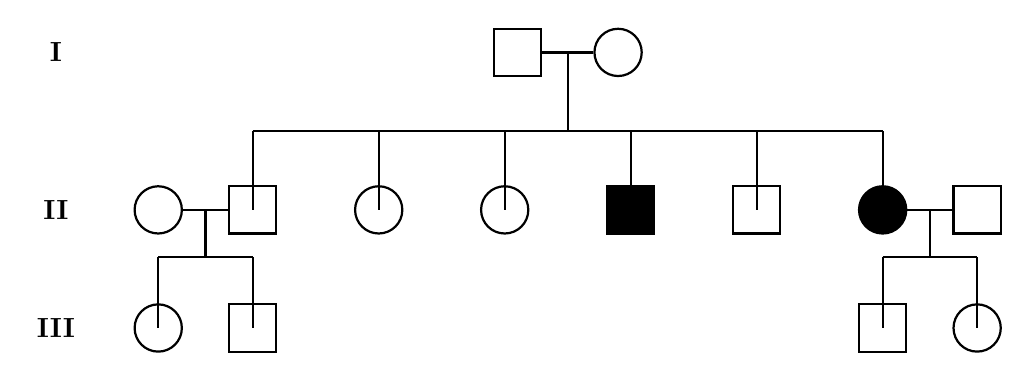
\begin{tikzpicture}[
    male/.style={rectangle,draw,minimum size=6mm,thick},
    female/.style={circle,draw,minimum size=6mm,thick},
    affected/.style={fill=black},
    mating/.style={draw,thick},
    sibling/.style={draw,thick}
  ]
    % Generation labels
    \node at (-6.5, 2) {\textbf{I}};
    \node at (-6.5, 0) {\textbf{II}};
    \node at (-6.5, -1.5) {\textbf{III}};
  
    % Generation I
    \node[male] (I1) at (-0.64, 2) {};
    \node[female] (I2) at (0.64, 2) {};
    \draw[thick] (I1) -- (I2);
    \coordinate (I-mid) at (0, 2);
    \coordinate (I-drop) at (0, 1);
    \draw[thick] (I-mid) -- (I-drop);
  
    % Sibling line for Gen II
    \draw[thick] (-4, 1) -- (4, 1);
  
    % Gen II Children connections
    \draw[thick] (-4, 1) -- (-4, 0);
    \draw[thick] (-2.4, 1) -- (-2.4, 0);
    \draw[thick] (-0.8, 1) -- (-0.8, 0);
    \draw[thick] (0.8, 1) -- (0.8, 0);
    \draw[thick] (2.4, 1) -- (2.4, 0);
    \draw[thick] (4, 1) -- (4, 0);
  
    % Gen II Nodes
    % 1st child (male) and spouse (female)
    \node[male] (II2) at (-4, 0) {};
    \node[female] (II1) at (-5.2, 0) {};
    \draw[thick] (II1) -- (II2);
    \coordinate (II-mid1) at (-4.6, 0);
    \coordinate (II-drop1) at (-4.6, -0.6);
    \draw[thick] (II-mid1) -- (II-drop1);
    \draw[thick] (-5.2, -0.6) -- (-4, -0.6);
    \draw[thick] (-5.2, -0.6) -- (-5.2, -1.5);
    \draw[thick] (-4, -0.6) -- (-4, -1.5);
    \node[female] (III1) at (-5.2, -1.5) {};
    \node[male] (III2) at (-4, -1.5) {};
  
    % 2nd and 3rd children (females)
    \node[female] (II3) at (-2.4, 0) {};
    \node[female] (II4) at (-0.8, 0) {};
  
    % 4th child (male, affected)
    \node[male, affected] (II5) at (0.8, 0) {};
  
    % 5th child (male)
    \node[male] (II6) at (2.4, 0) {};
  
    % 6th child (female, affected) and spouse (male)
    \node[female, affected] (II7) at (4, 0) {};
    \node[male] (II8) at (5.2, 0) {};
    \draw[thick] (II7) -- (II8);
    \coordinate (II-mid2) at (4.6, 0);
    \coordinate (II-drop2) at (4.6, -0.6);
    \draw[thick] (II-mid2) -- (II-drop2);
    \draw[thick] (4, -0.6) -- (5.2, -0.6);
    \draw[thick] (4, -0.6) -- (4, -1.5);
    \draw[thick] (5.2, -0.6) -- (5.2, -1.5);
    \node[male] (III3) at (4, -1.5) {};
    \node[female] (III4) at (5.2, -1.5) {};
  
  \end{tikzpicture}
  \end{center}

  \item Enlist the major structures observed in developing human embryo, which replicates its phylogenetic lineage.\pts{4}
  \item Explain how lethal alleles disrupt Mendelian phenotypic ratios.\pts{2}
\end{parts}

\medskip\noindent\textbf{Question 4.} Answer the following parts:
\begin{parts}
  \item Illustrate meiotic consequences in an individual heterozygous for a reciprocal translocation.\pts{6}
  \item Matings between purple starfish of identical genotype produced offspring as follows: 18 pink, 54 purple, and 24 albino.
  \begin{parts}
    \item What epistatic ratio is shown by these offsprings?\pts{3}
    \item What are the genotypes of the parents and the offspring (use your own symbols)?\pts{3}
  \end{parts}
\end{parts}

\pagebreak
\begin{center}
  \textbf{SECTION -- B} \\
  \textbf{(Economic Zoology) (Marks: 35)}
\end{center}

\smallskip
\noindent\textit{Note: Answer three questions including, Question No. 1 which is compulsory.}

\bigskip
\noindent\textbf{Question 1.} Answer the following parts:
\begin{parts}
  \item Define the following:\pts{$1 \times 2 = 2$}
  \begin{parts}
    \item Smart milk
    \item Propolis
  \end{parts}

  \item State whether the following statements are True or False. Justify your answer in 2--3 sentences:\pts{$2 \times 3 = 6$}
  \begin{parts}
    \item Worker honey bees are produced from the fertile eggs laid by the queen.
    \item Pebrine is the disease of silk.
    \item Lac is produced in large quantities by male lac insect.
  \end{parts}

  \item Answer the following:\pts{$1 \times 3 = 3$}
  \begin{parts}
    \item Name any two breeds of indigenous cow.
    \item Name any two species of exotic fish.
    \item Name any two diseases of poultry.
  \end{parts}
\end{parts}

\medskip\noindent\textbf{Question 2.} Answer the following parts:
\begin{parts}
  \item Describe various types of cattle sheds and their advantages.\pts{6}
  \item Write a note on sericulture.\pts{6}
\end{parts}

\medskip\noindent\textbf{Question 3.} Answer the following parts:
\begin{parts}
  \item Give an account of induced breeding in fish.\pts{6}
  \item Describe the different housing systems in poultry farming.\pts{6}
\end{parts}

\medskip\noindent\textbf{Question 4.} Write short notes on the following:\pts{$4 \times 3 = 12$}
\begin{parts}
  \item Lac processing and its uses
  \item Various castes of honey bee
  \item Pearl formation in natural condition.
\end{parts}

\vfill
\rule{\linewidth}{0.4pt}
\begin{center}\small
\href{https://bhu-exam.vercel.app/}{Click Here}\\[4pt]\href{https://me-aryan.vercel.app/}{Click Here}\\[4pt]\href{https://quashan-me.vercel.app/}{Click Here}
\end{center}

\end{document}
